\documentclass[a4paper, 11pt]{beamer}
\usepackage[utf8]{inputenc}
\usepackage[T1]{fontenc}
\usepackage[english]{babel}
\usepackage{graphicx}

\usetheme{Warsaw}

\title{KAMISADO}
\author{Valentin BENOZILLO, Mathieu VIOLA, Rémi VIOLA}
\date{\today}

\begin{document}

\begin{frame}
 \titlepage
\end{frame}

\begin{frame}
 \tableofcontents
\end{frame}

\begin{frame}
 \frametitle{Kamisado}
 \begin{center}
  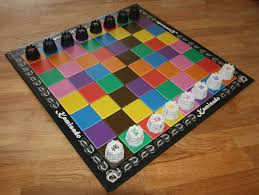
\includegraphics[scale = 0.07]{kamisado.jpeg}
 \end{center}
\end{frame}

\section{The game}
\begin{frame}
 \frametitle{Kamisado}
 \begin{center}
  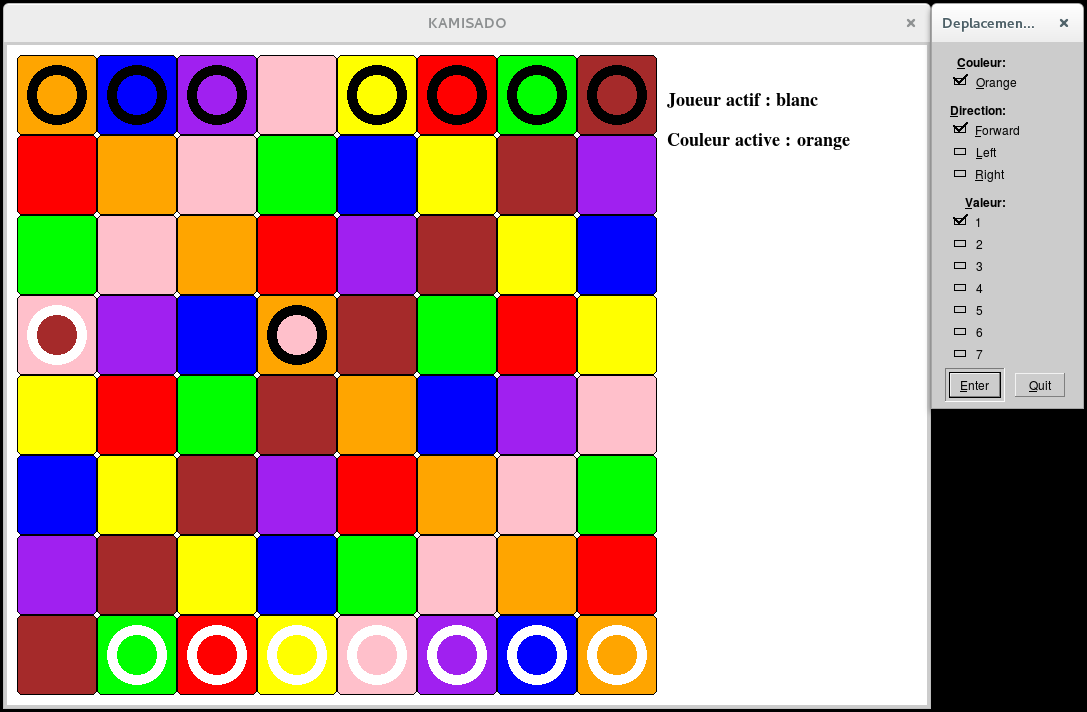
\includegraphics[scale = 0.25]{kamisado.png}
 \end{center}
\end{frame}

\section{The division of the work}
\begin{frame}
 \frametitle{The division of the work}
 \begin{itemize}
  \item Basics of the game by Rémi (k.pl)
  \item Graphical user interface by Rémi (k.pl)
  \item Artificial intelligences by all of us (ia\_firstname.pl)
 \end{itemize}
\end{frame}

\section{The heuristics}
\subsection{Heuristic remi}
\begin{frame}
 \frametitle{The heuristics}
 \framesubtitle{Heuristic remi}
 \begin{table}[htbp]
  \centering
  \begin{tabular}{c c}
    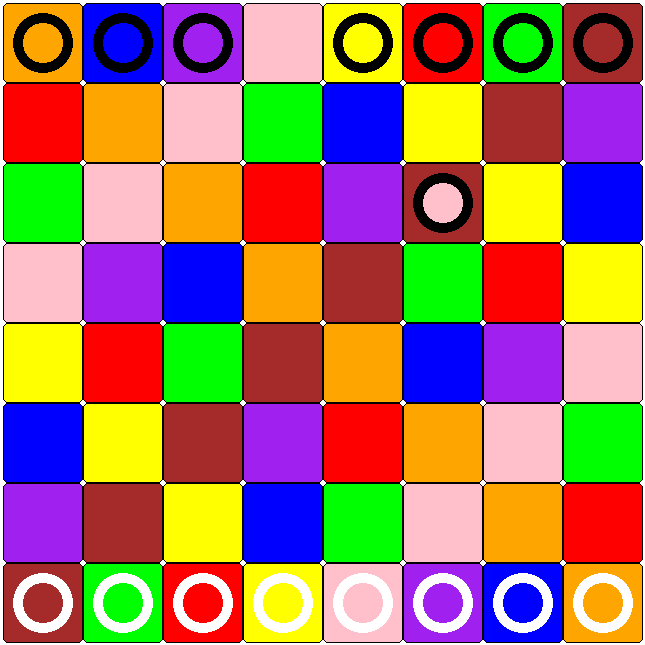
\includegraphics[scale = 0.11]{remi1b.png} & 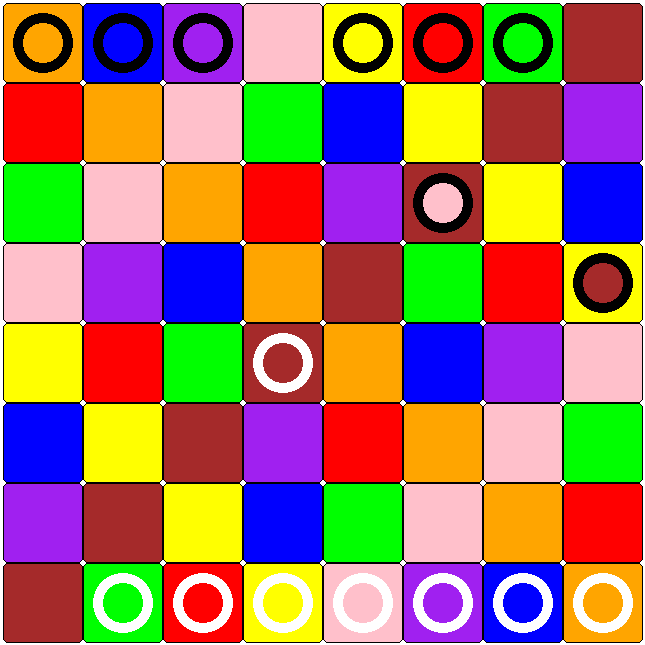
\includegraphics[scale = 0.11]{remi2b.png} \\
    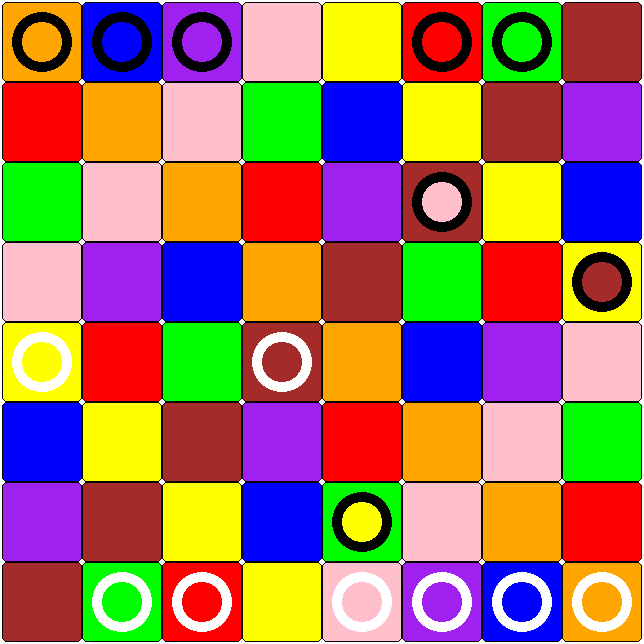
\includegraphics[scale = 0.11]{remi3b.png} & 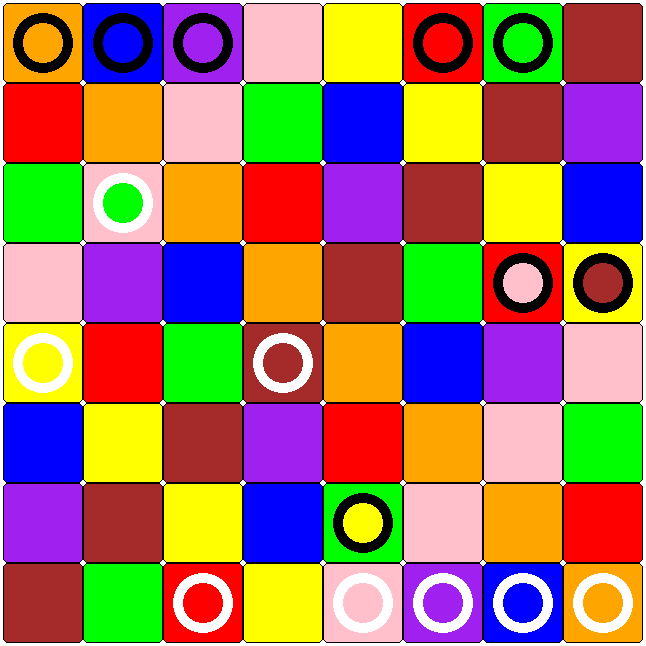
\includegraphics[scale = 0.11]{remi4b.png} \\
  \end{tabular}
  \caption{Four first rounds of a game where AI starts}
 \end{table}
\end{frame}

\subsection{Heuristic valentin}

\begin{frame}
\frametitle{The heuristics}
\framesubtitle{Heuristic valentin}
\begin{center}

	\begin{tabular}{c c}
     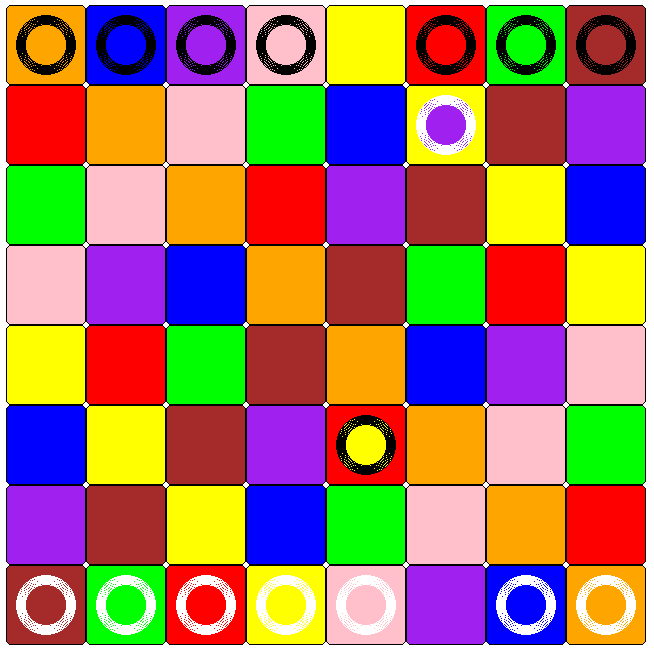
\includegraphics[scale = 0.12]{val1.png} &
     \pause
     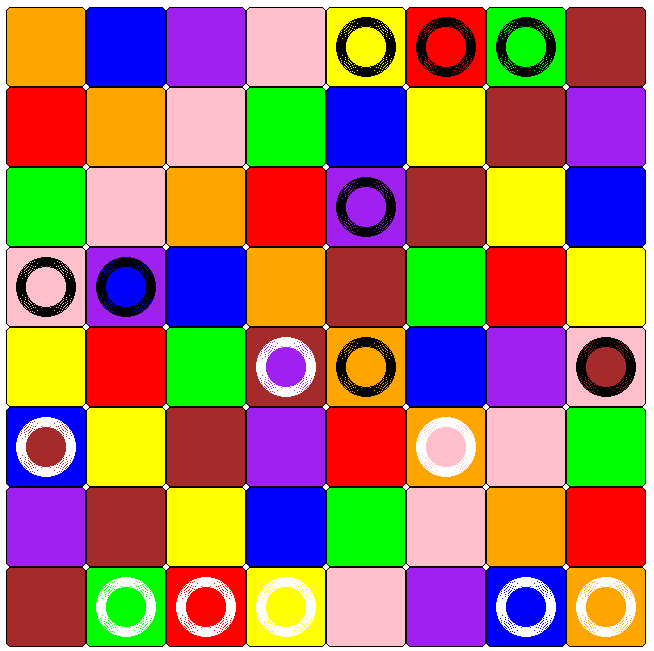
\includegraphics[scale = 0.12]{val2.png}\\
   \end{tabular}
   \end{center}
\end{frame}

\begin{frame}
\frametitle{The heuristics}
\framesubtitle{Heuristic valentin}
\begin{center}

	\begin{tabular}{c c c}
     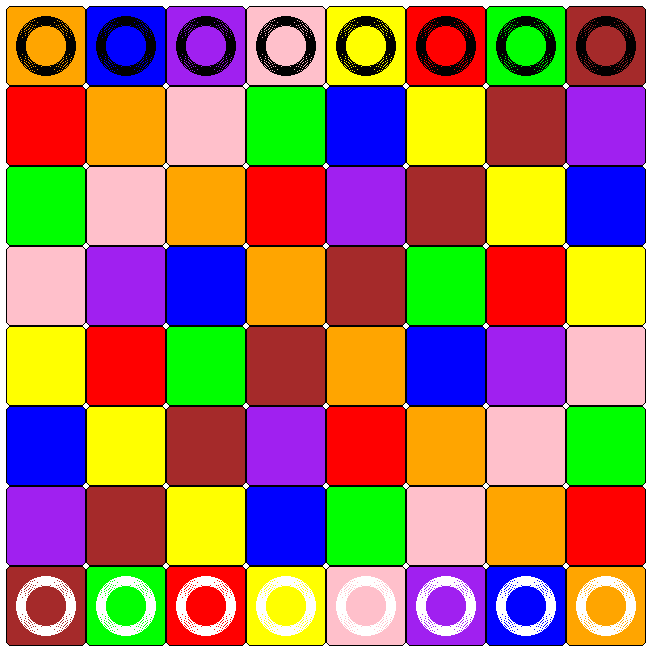
\includegraphics[scale = 0.12]{val_1.png} &
     \pause
     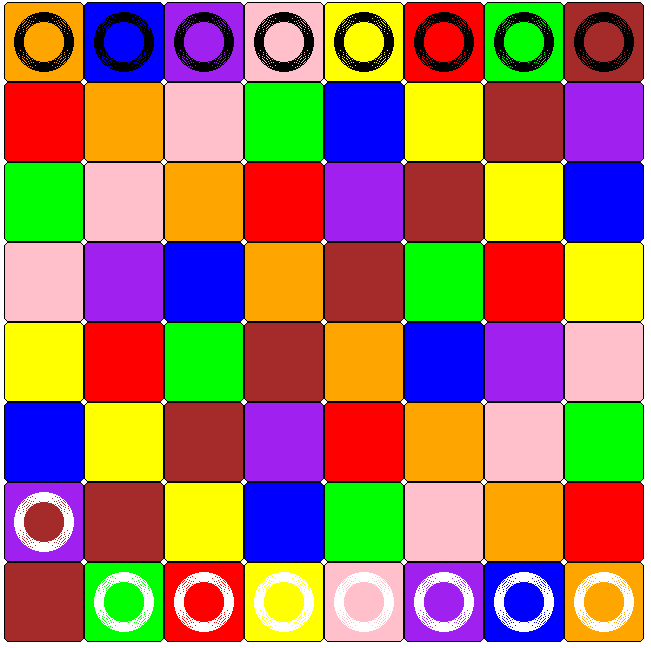
\includegraphics[scale = 0.12]{val_2.png} &
     \pause
    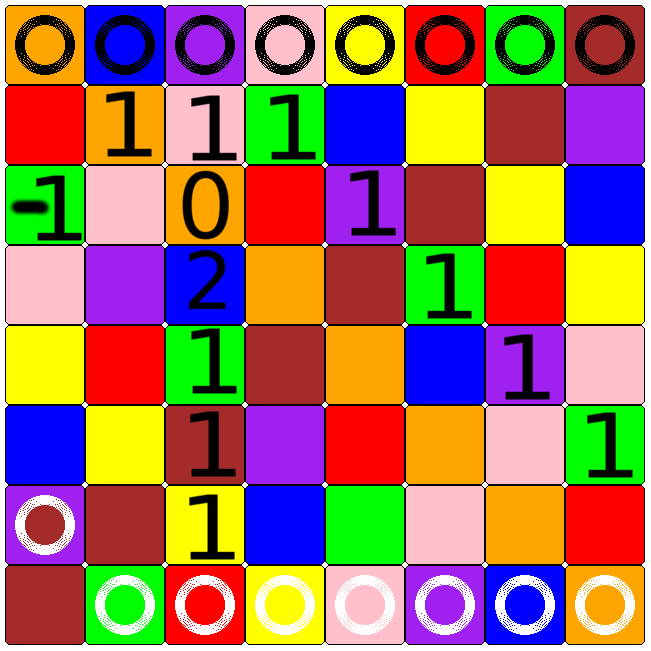
\includegraphics[scale = 0.12]{val_3.png} \\
    \pause
    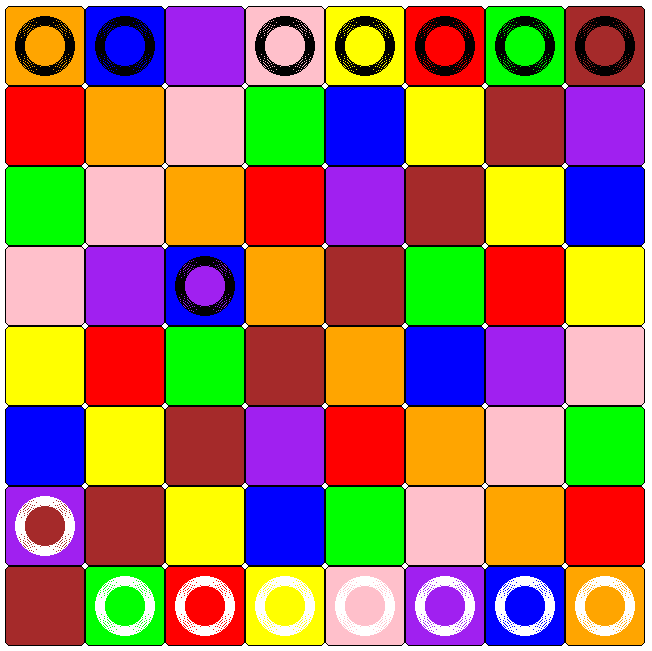
\includegraphics[scale = 0.12]{val_4.png} &
    \pause
    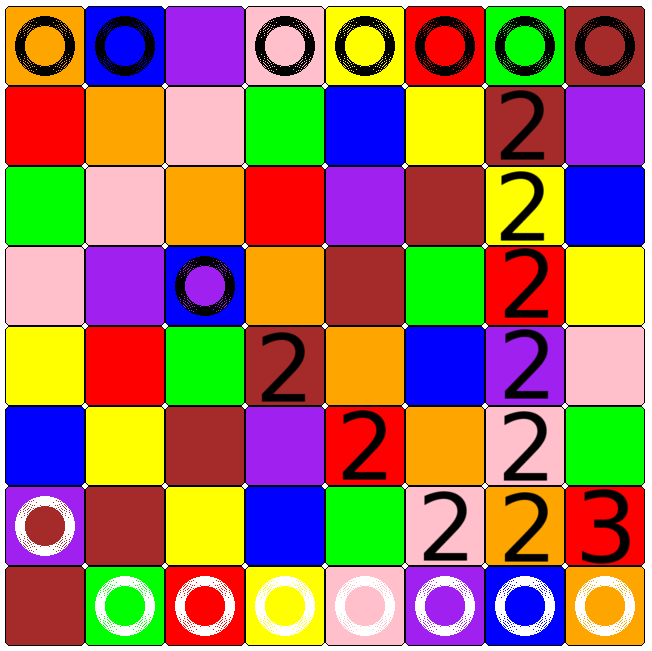
\includegraphics[scale = 0.12]{val_5.png} &
    \pause
    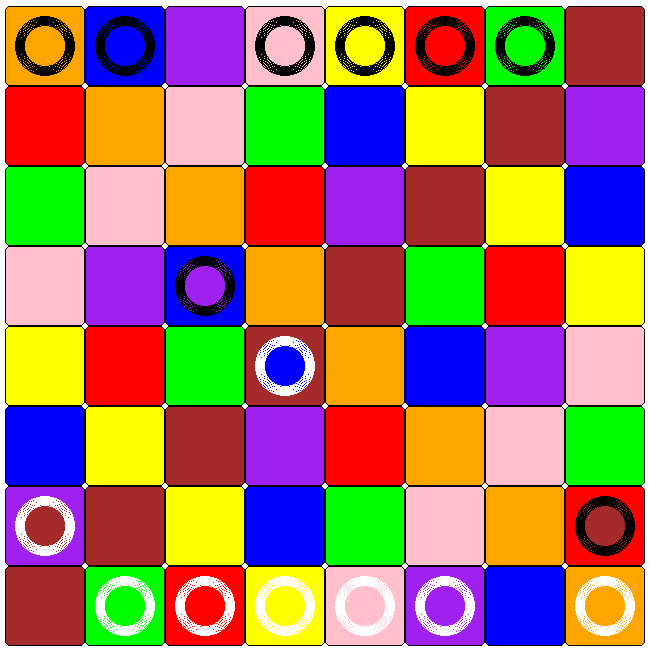
\includegraphics[scale = 0.12]{val_6.png} \\
   \end{tabular}
   
\end{center}
\end{frame}

\subsection{Heuristic mathieu}
\begin{frame}
 \frametitle{The heuristics}
 \framesubtitle{Heuristic mathieu}
 \begin{table}[htbp]
  \centering
  \begin{tabular}{c c}
    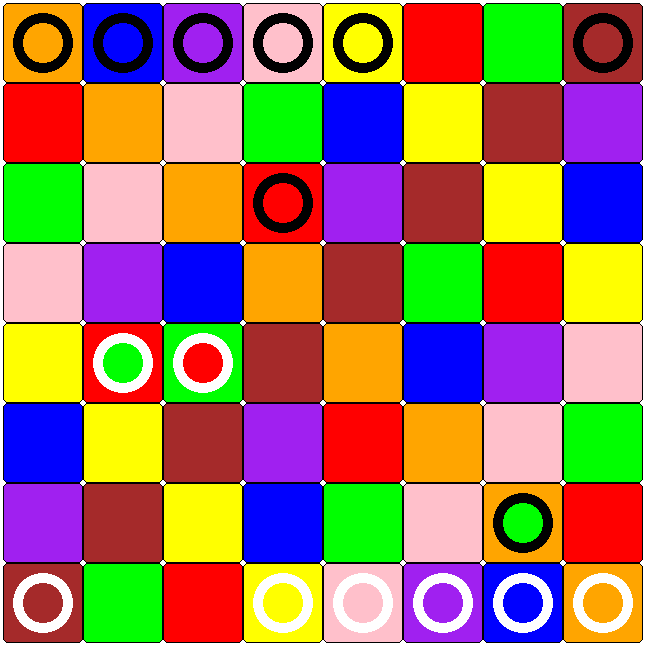
\includegraphics[scale = 0.11]{mathieu_2.png} & 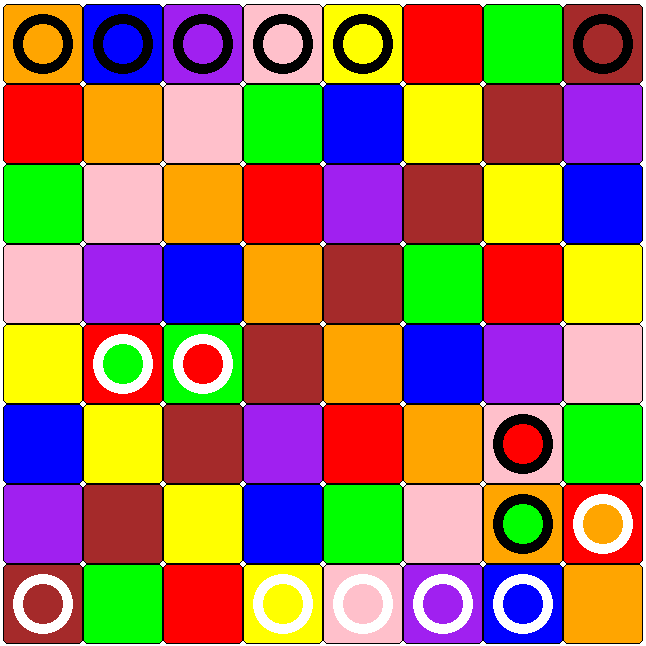
\includegraphics[scale = 0.11]{mathieu_3.png} \\
    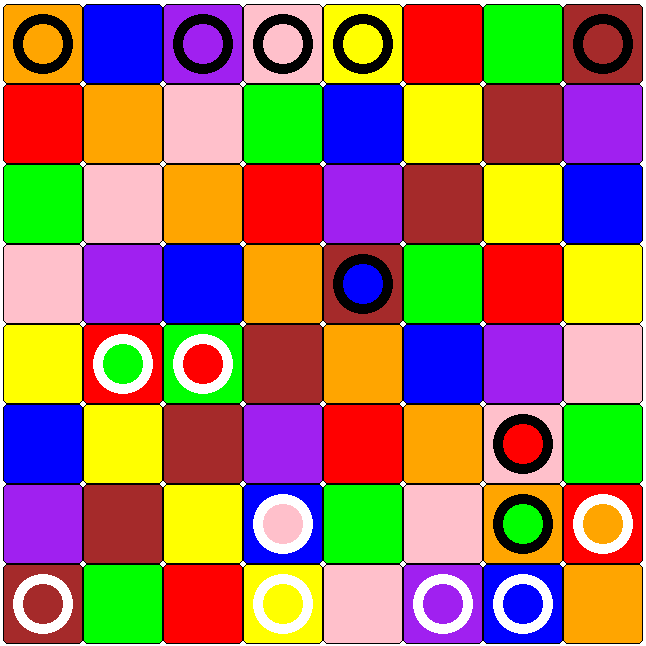
\includegraphics[scale = 0.11]{mathieu_4.png} & 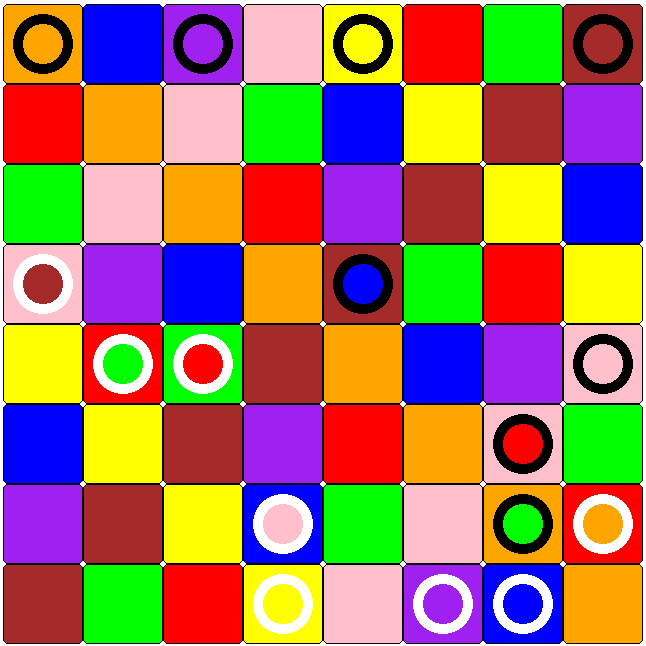
\includegraphics[scale = 0.11]{mathieu_5.png} \\
  \end{tabular}
  \caption{Four rounds of a game after green-forward-3}
 \end{table}
\end{frame}

\subsection{Heuristic mathieu2}
\begin{frame}
 \frametitle{The heuristics}
 \framesubtitle{Heuristic mathieu2}
 \begin{table}[htbp]
  \centering
  \begin{tabular}{c c}
    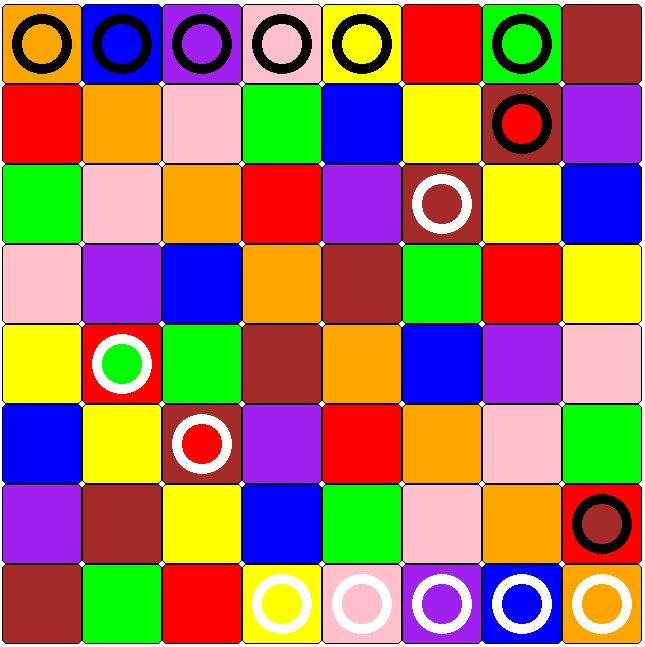
\includegraphics[scale = 0.11]{mathieu2_3.png} & 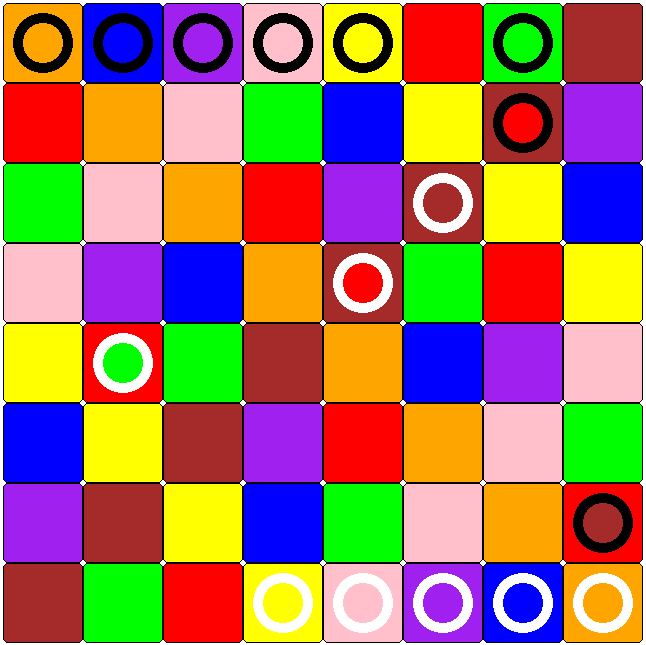
\includegraphics[scale = 0.11]{mathieu2_4.png} \\
    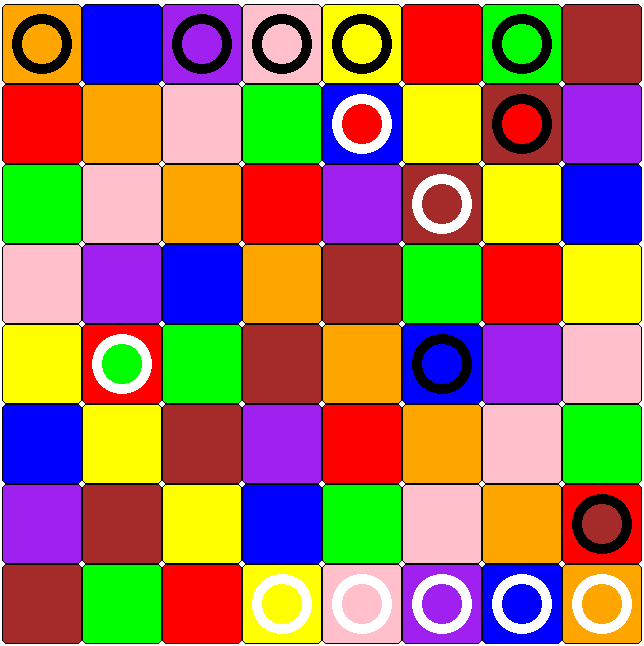
\includegraphics[scale = 0.11]{mathieu2_5.png} & 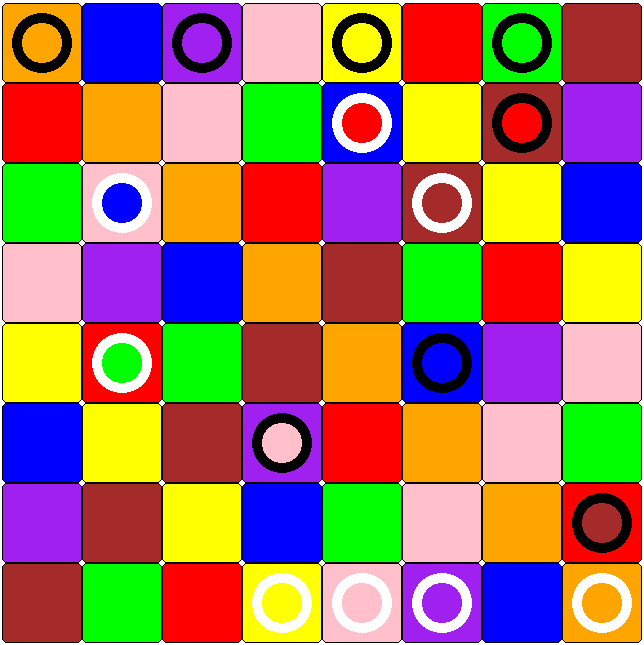
\includegraphics[scale = 0.11]{mathieu2_6.png} \\
  \end{tabular}
  \caption{Four rounds of a game after green-forward-3}
 \end{table}
\end{frame}

\subsection{Heuristic mathieu3}
\begin{frame}
 \frametitle{The heuristics}
 \framesubtitle{Heuristic mathieu3}
 \begin{table}[htbp]
  \centering
  \begin{tabular}{c c}
    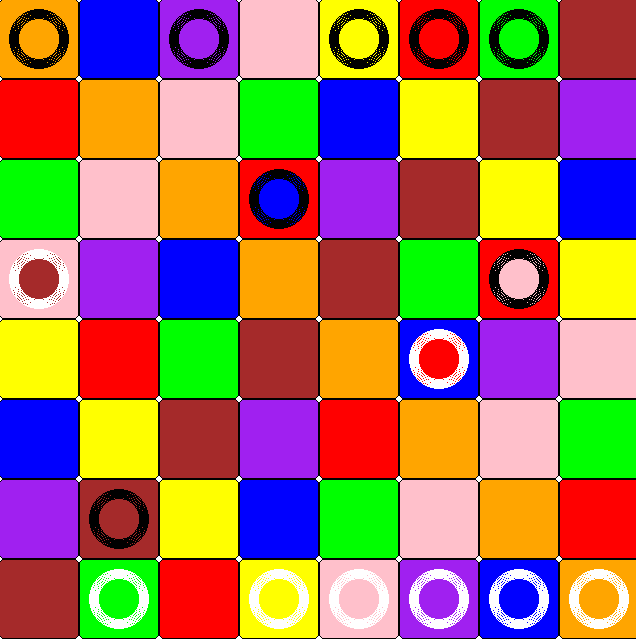
\includegraphics[scale = 0.11]{mathieu3_1.png} & 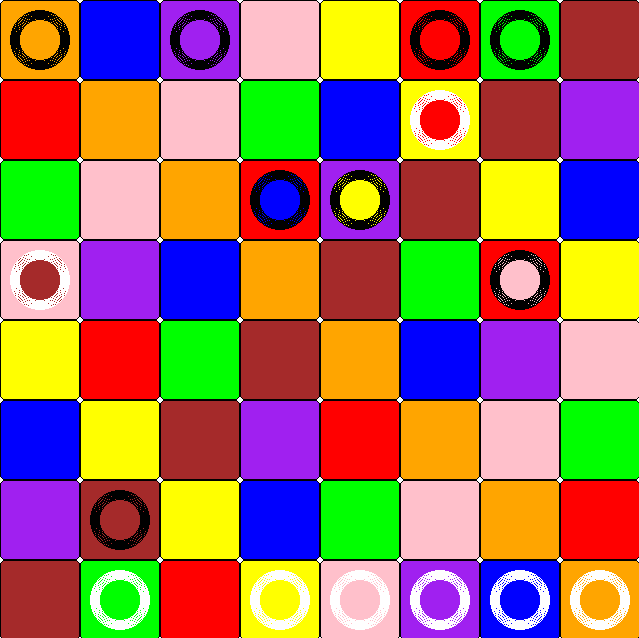
\includegraphics[scale = 0.11]{mathieu3_2.png} \\
    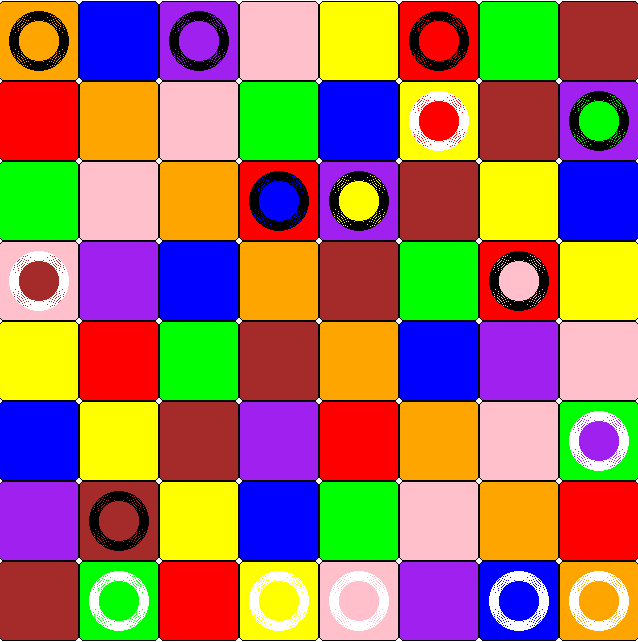
\includegraphics[scale = 0.11]{mathieu3_3.png} & 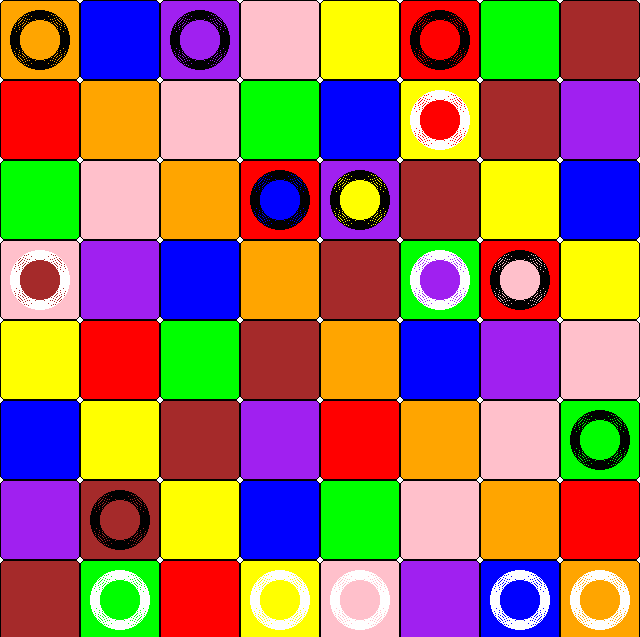
\includegraphics[scale = 0.11]{mathieu3_4.png} \\
  \end{tabular}
  \caption{Four rounds of a game after IA starts}
 \end{table}
 
\end{frame}

\subsection{Heuristic mathieu4}
\begin{frame}
 \frametitle{The heuristics}
 \framesubtitle{Heuristic mathieu4}
 
 \begin{table}[htbp]
  \centering
  \begin{tabular}{c c}
    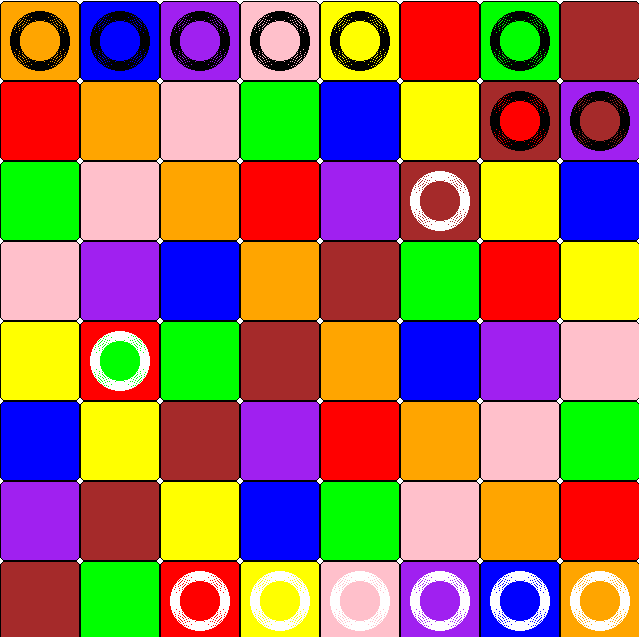
\includegraphics[scale = 0.11]{mathieu4_1.png} & 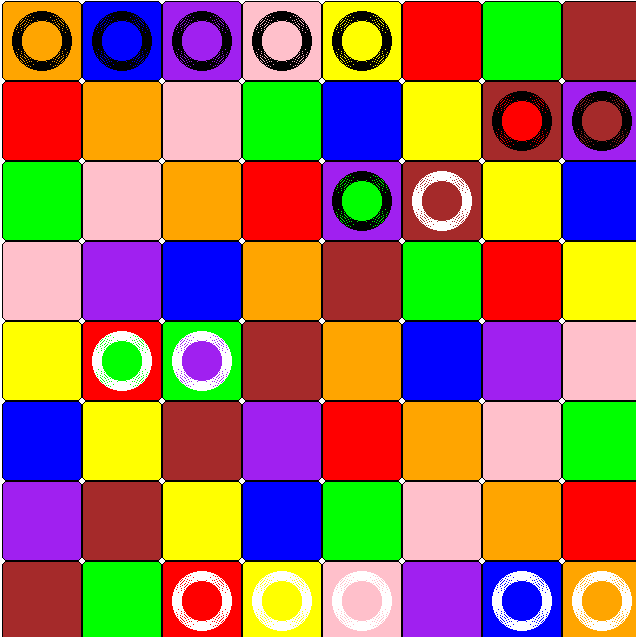
\includegraphics[scale = 0.11]{mathieu4_2.png} \\
    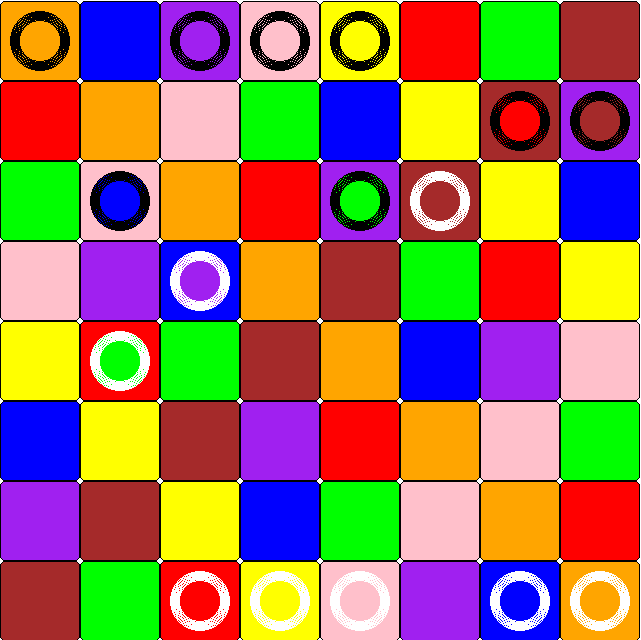
\includegraphics[scale = 0.11]{mathieu4_3.png} & 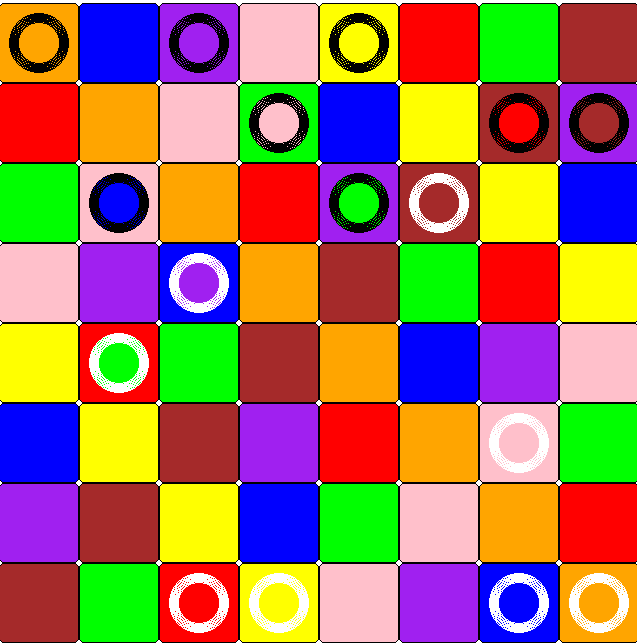
\includegraphics[scale = 0.11]{mathieu4_4.png} \\
  \end{tabular}
  \caption{Four rounds of a game after green-forward-3}
 \end{table}
\end{frame}

\section{The balance sheet}
\subsection{Negative points}
\begin{frame}
 \frametitle{The balance sheet}
 \framesubtitle{Negative points}
 \begin{itemize}
  \item Graphical user interface : Not rather intuitive and ergonomic
  \pause
  \item Lack of tests between artificial intelligences
  \pause
  \item Draw issue
 \end{itemize}
\end{frame}

\subsection{Positive points}
\begin{frame}
 \frametitle{The balance sheet}
 \framesubtitle{Positive points}
 \begin{itemize}
  \item Artificial intelligences rather fast and effective
  \pause
  \item Scalable
  \pause
  \item Only prolog
 \end{itemize}
\end{frame}

\end{document}
